\chapter{一些使用技巧}



\section{软件使用技巧}

如果在生成文档时发生错误,不要惊慌,可以先把生成的文件全部删除再试一次。
就是把除了tex文件外的其它同名文件都删掉。

使用WinEdt编辑tex文件时,如果嫌命令太长打着费劲,试试只输前几个字母然后按
“Ctrl+Enter”键,哈!WinEdt替你把剩下的部分补全了。

遇到问题不要慌,看下方小窗口里提示的出错信息,会有很多提示你错在哪里的。

不同系统下生成的eps可能会有兼容问题,
如本模版中的setroot.eps和rffndb.eps,在xp和windows 7 x64似乎不能通用。
解决方案很简单,
只要用bmeps -p 1 -c setroot.jpg setrooteps重新生成一次即可解决。
rffndb.eps生成命令同setroot.eps。

这个文档我用的是gVim编辑的,gVim自带的自动补全功能比WinEdt更强大,让我在
编写这个文档时省了不少重复工作量。

如果会使用make程序,那么使用Makefile来生成文档更方便一些。

在UTF-8版本中,如果一个命令后紧跟汉字,比如像这样“\verb+songti好的+”,
编译的时候就会报错,处理办法就是在命令后面加一个空格或者一个大括号,就像这样:
“\verb+songti 好的+”或者“\verb+songti{}好的+”

差不多了,就写这几条吧,想起来什么再写。

把另外几个参考文献当引用例子使用一下:专利\cite{WangZL},标准\cite{WangStd},
电子文档\cite{ZLB:1997},期刊文章\cite{LUOZ:2007},
学位论文\cite{wang:2008,wangmt:2008}。

这份文档从规划到完成,历时近20日,也是自己\LaTeX 学习一个总结吧。

\section{推荐的\TeX 准所见所得编辑器}

如果使用\XeTeX ,那么推荐一个强大的所见所得\TeX 准所见所得编辑器 TeXstudio。
该软件的优点有:

\begin{enumerate}
	
	\item{跨平台软件,可在Windows, MacOS,Linux上安装运行}
	
	\item{有中文语言包界面} 
	
	\item{可以在源码与pdf间关联跳跃,实现准“所见即所得”} 
	
\end{enumerate}

将TeXstudio的默认构建命令改为:XeLaTeX,如图\ref{Construct}所示。

\begin{figure}[th]
	\centering
	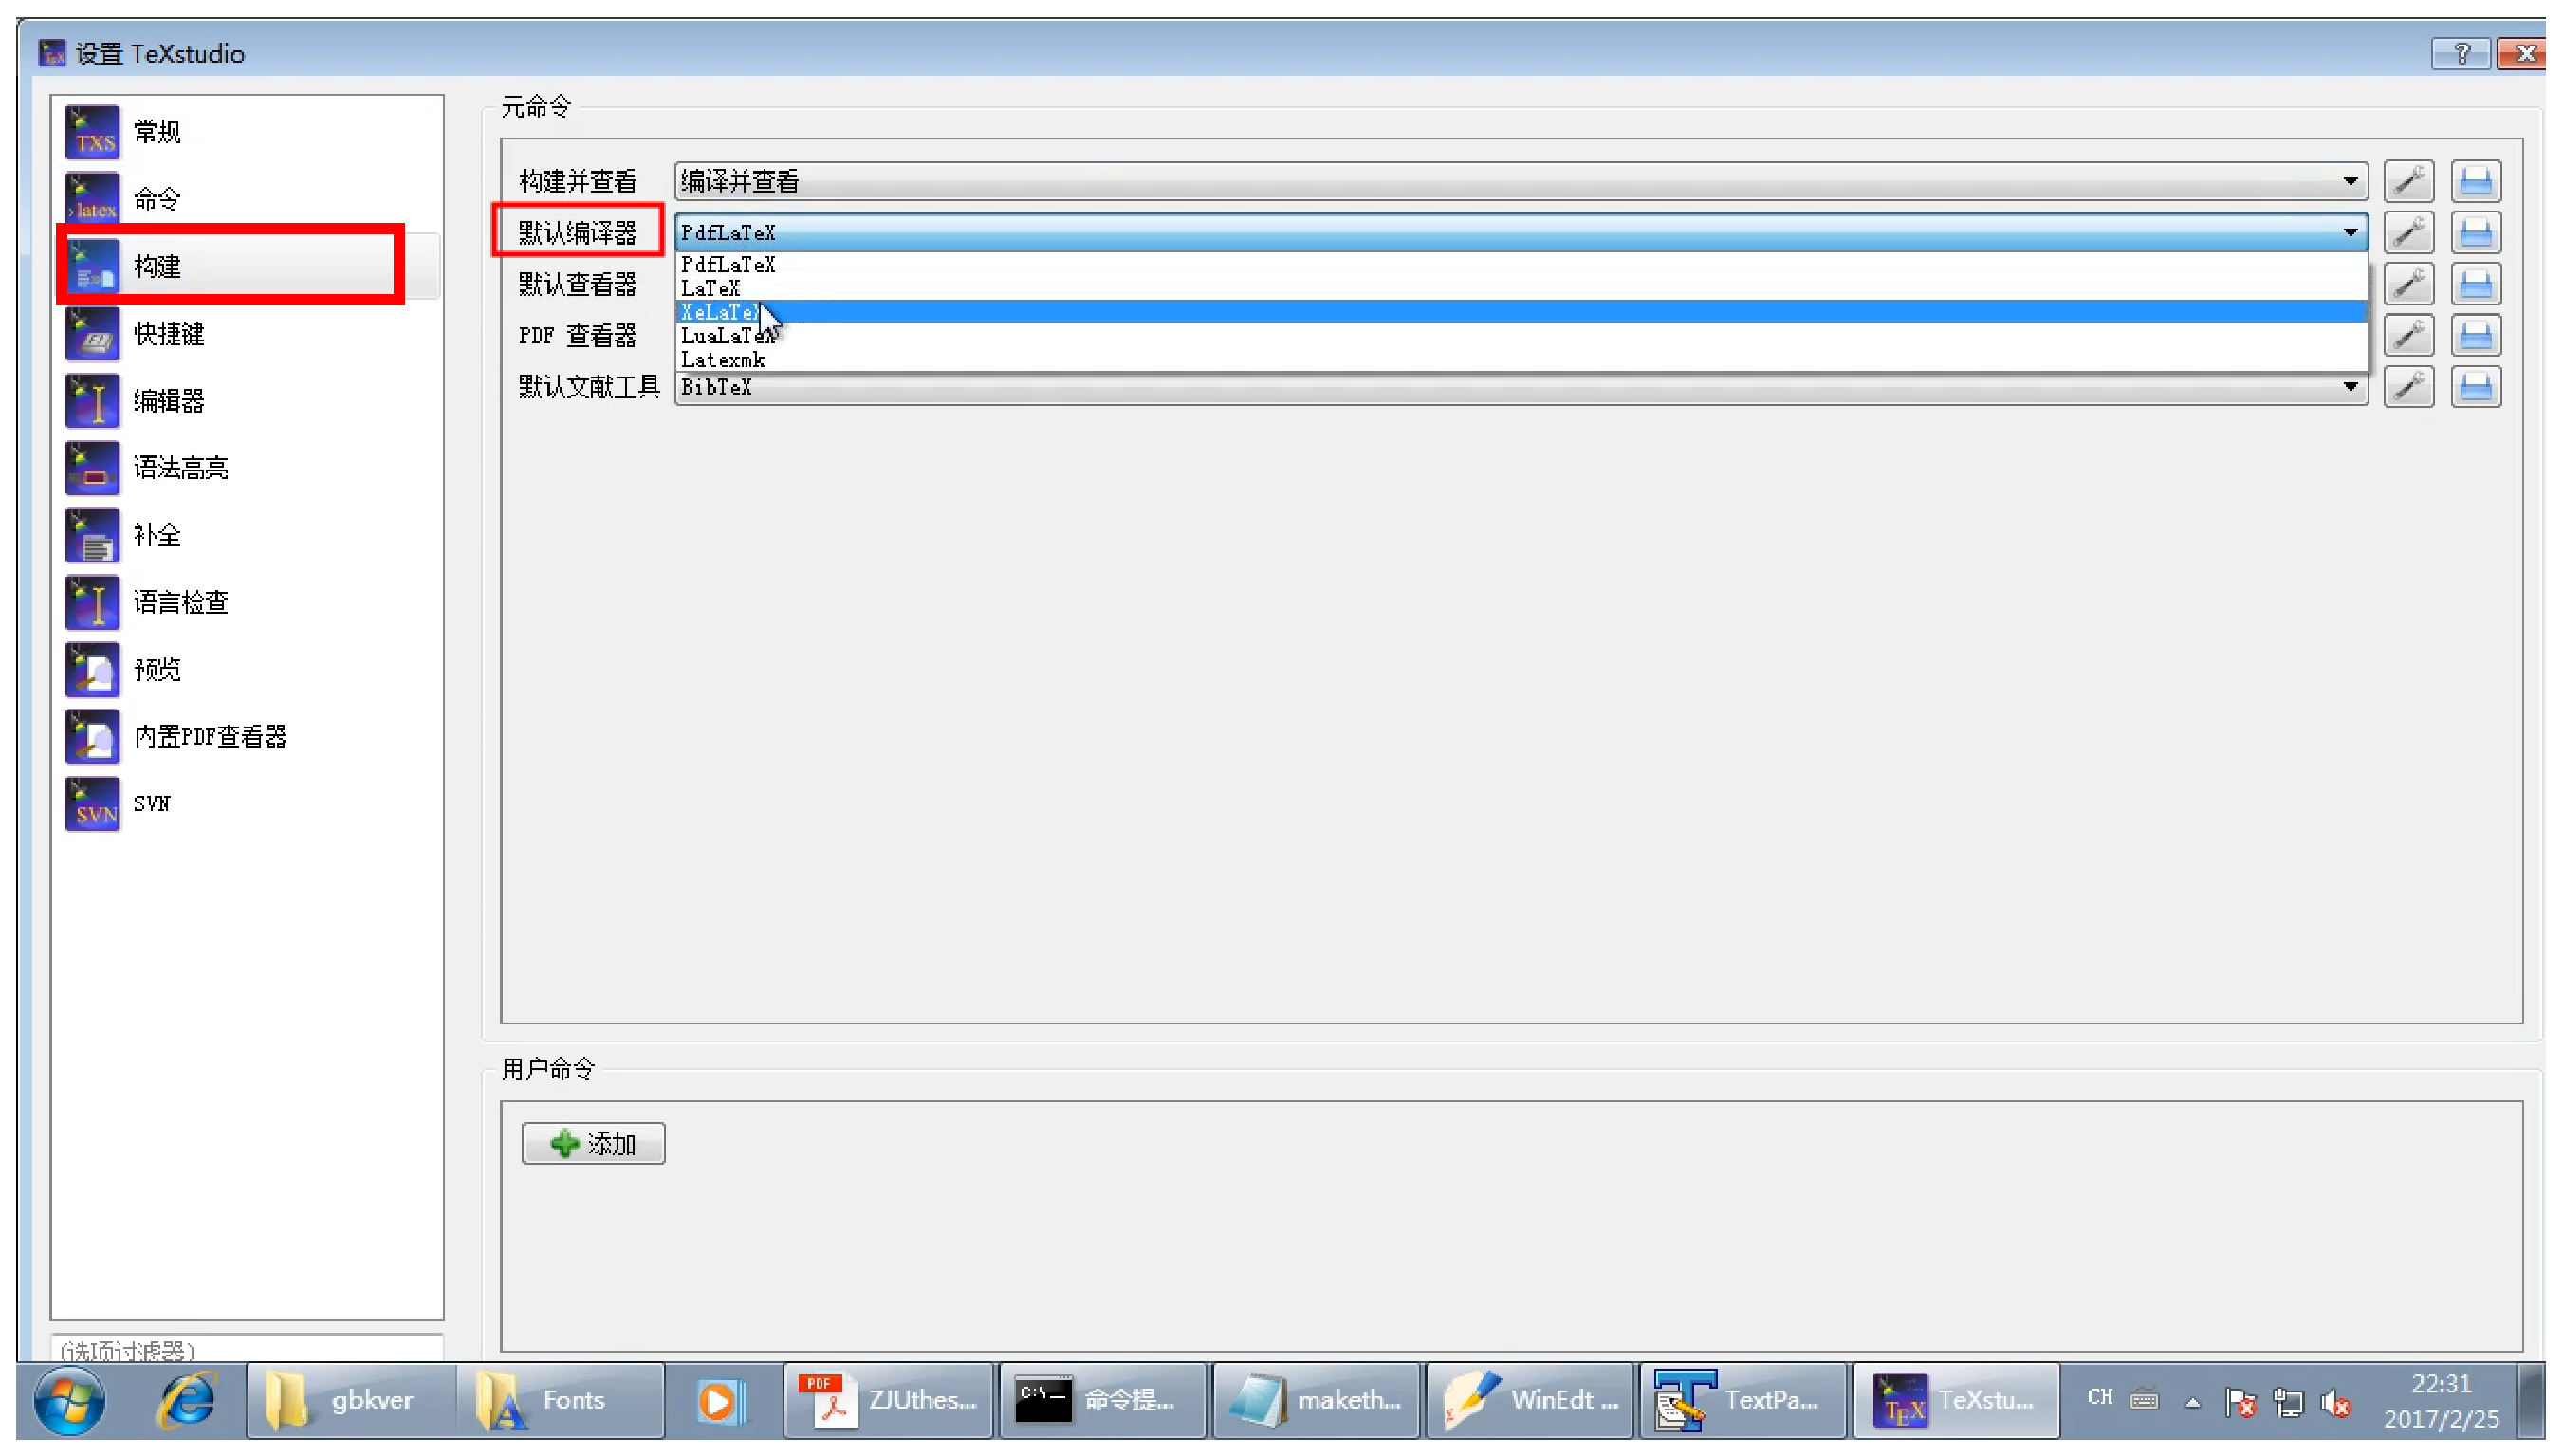
\includegraphics[width=\textwidth]{./Pictures/Construct.eps}\\
	\caption{修改TeXstudio的默认构建命令}
	\label{Construct}
\end{figure}

这样,在使用TeXstudio生成pdf,并打开右侧pdf预览后,就可以使用“Ctrl+鼠标左键”
实现源码与pdf显示之间的来回跳转功能了。

\newpage

从pdf跳转到tex源码,如图\ref{pdftotex}所示。

\begin{figure}[th]
	\centering
	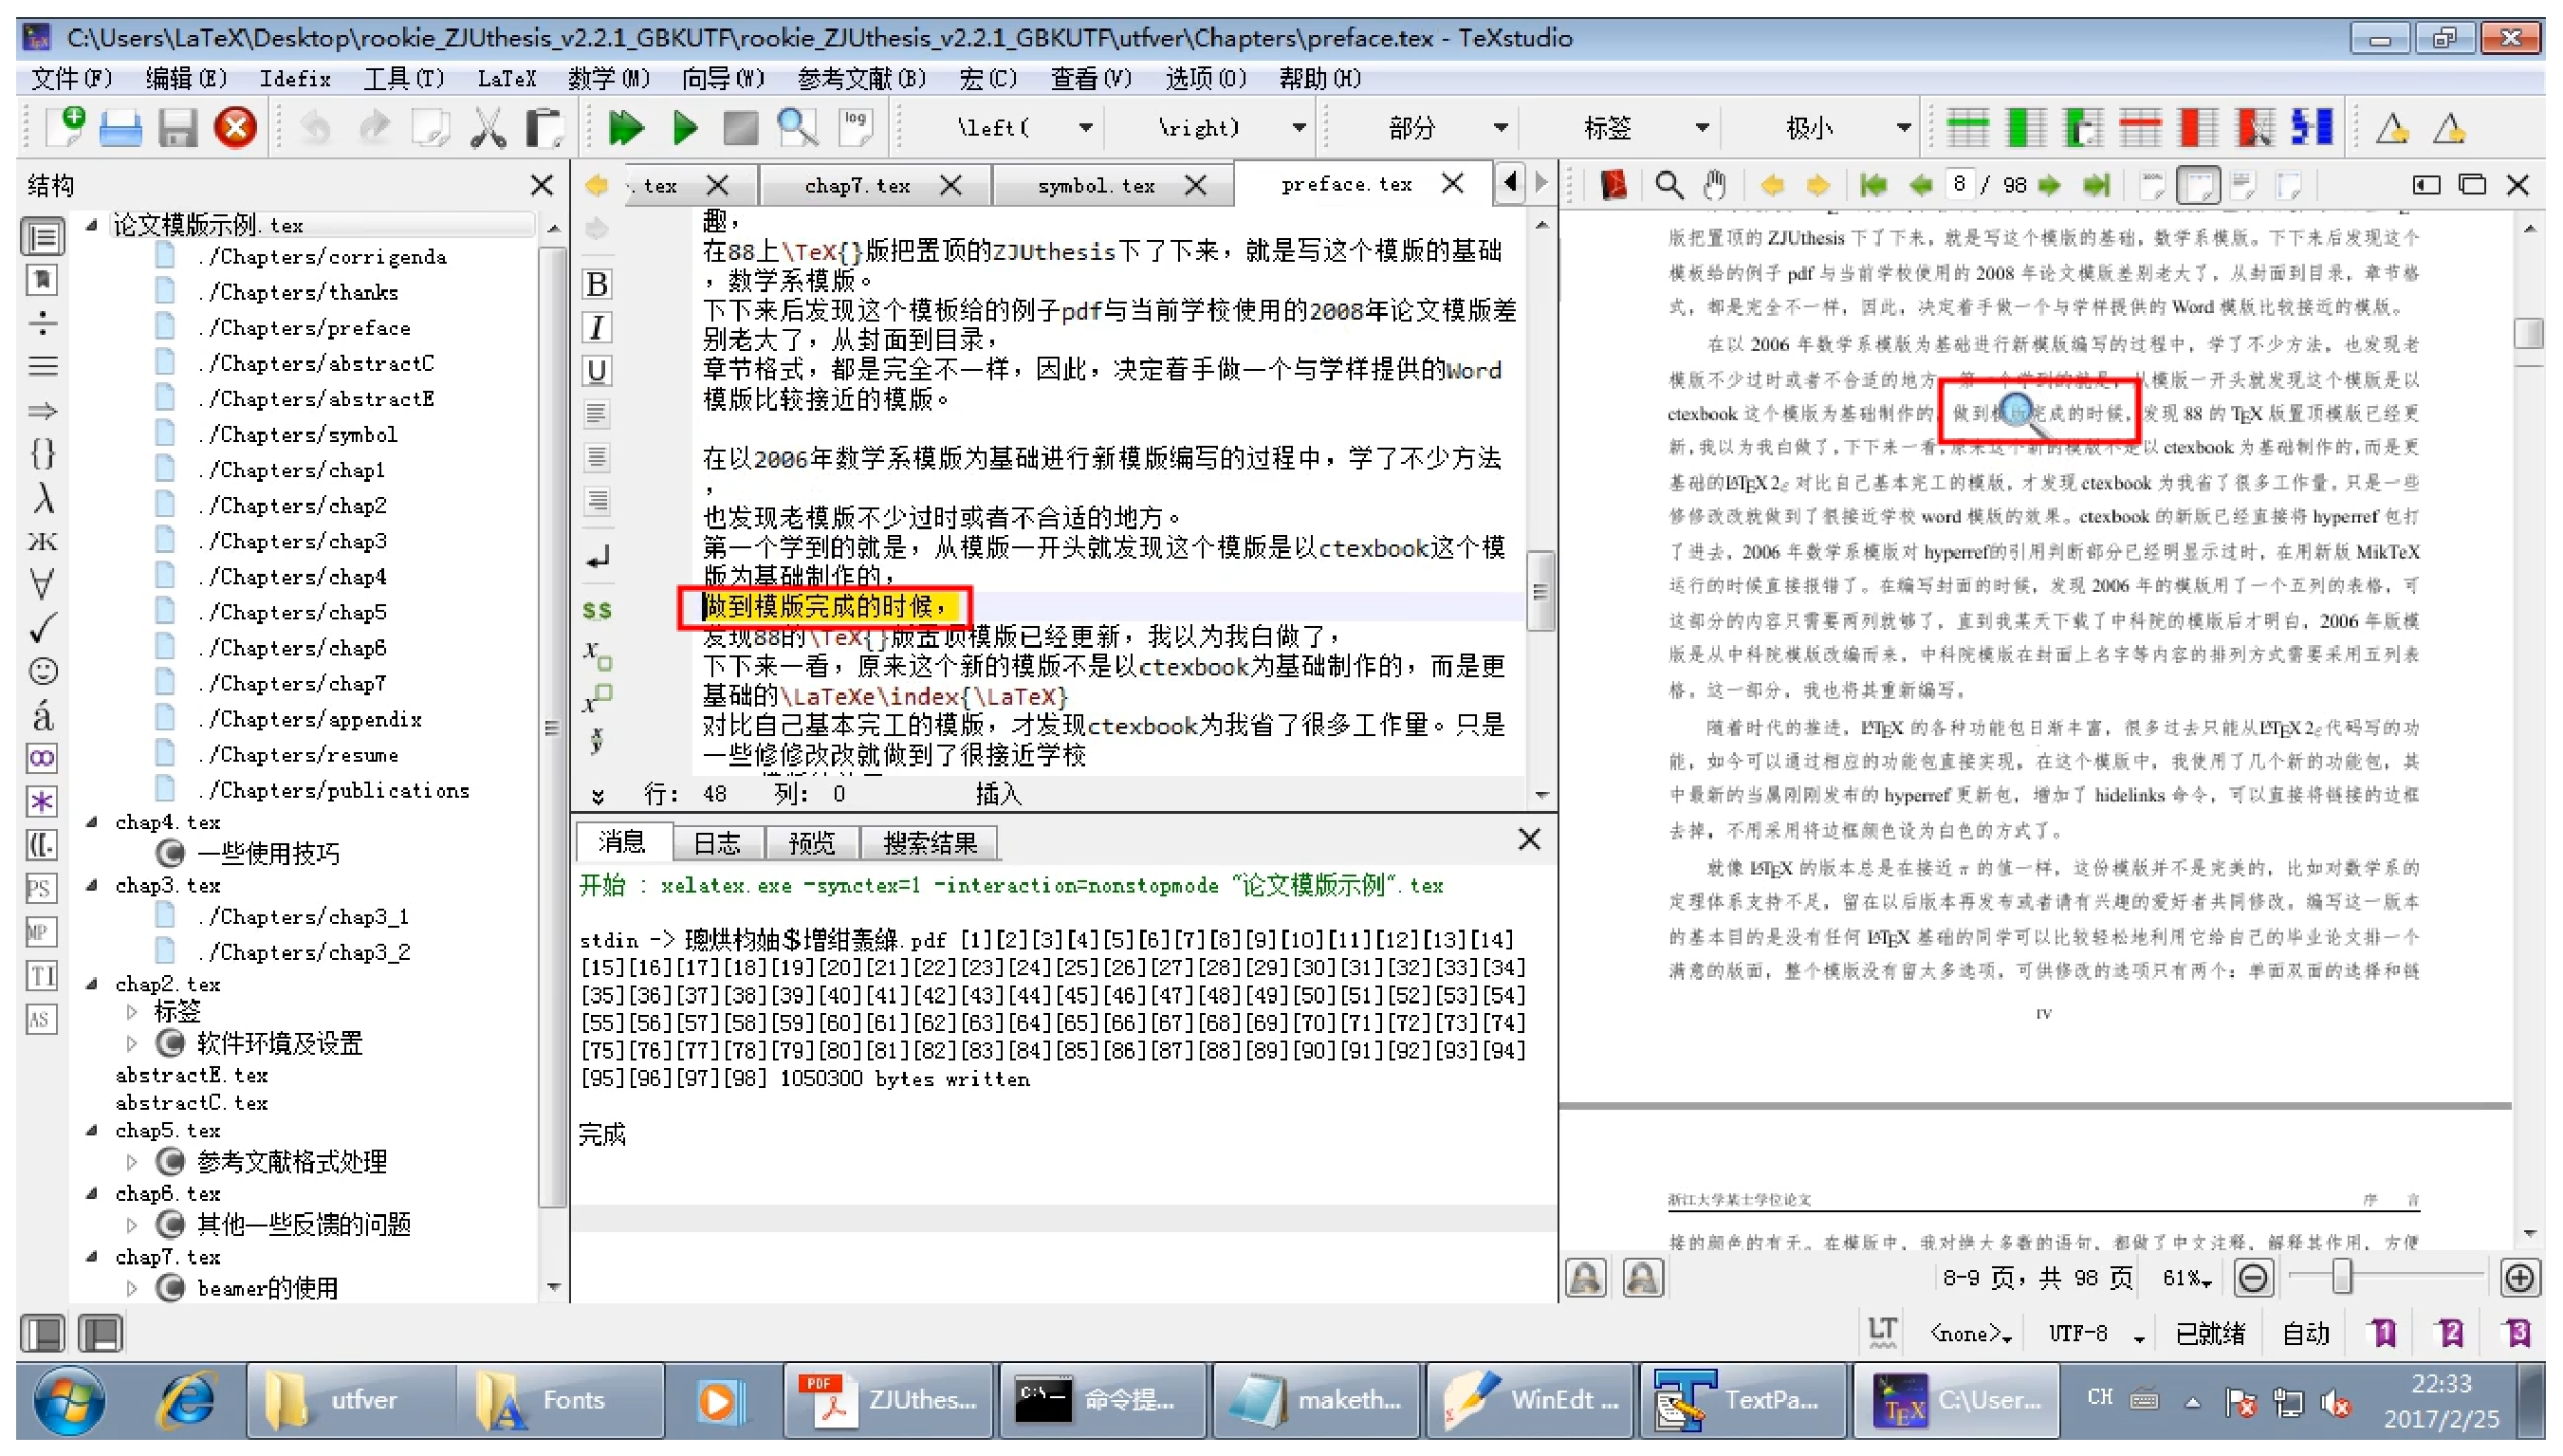
\includegraphics[width=\textwidth]{./Pictures/pdftotex.eps}\\
	\caption{TeXstudio中从pdf跳转到tex源码}
	\label{pdftotex}
\end{figure}

从tex源码跳转到pdf,如图\ref{textopdf}所示。

\begin{figure}[th]
	\centering
	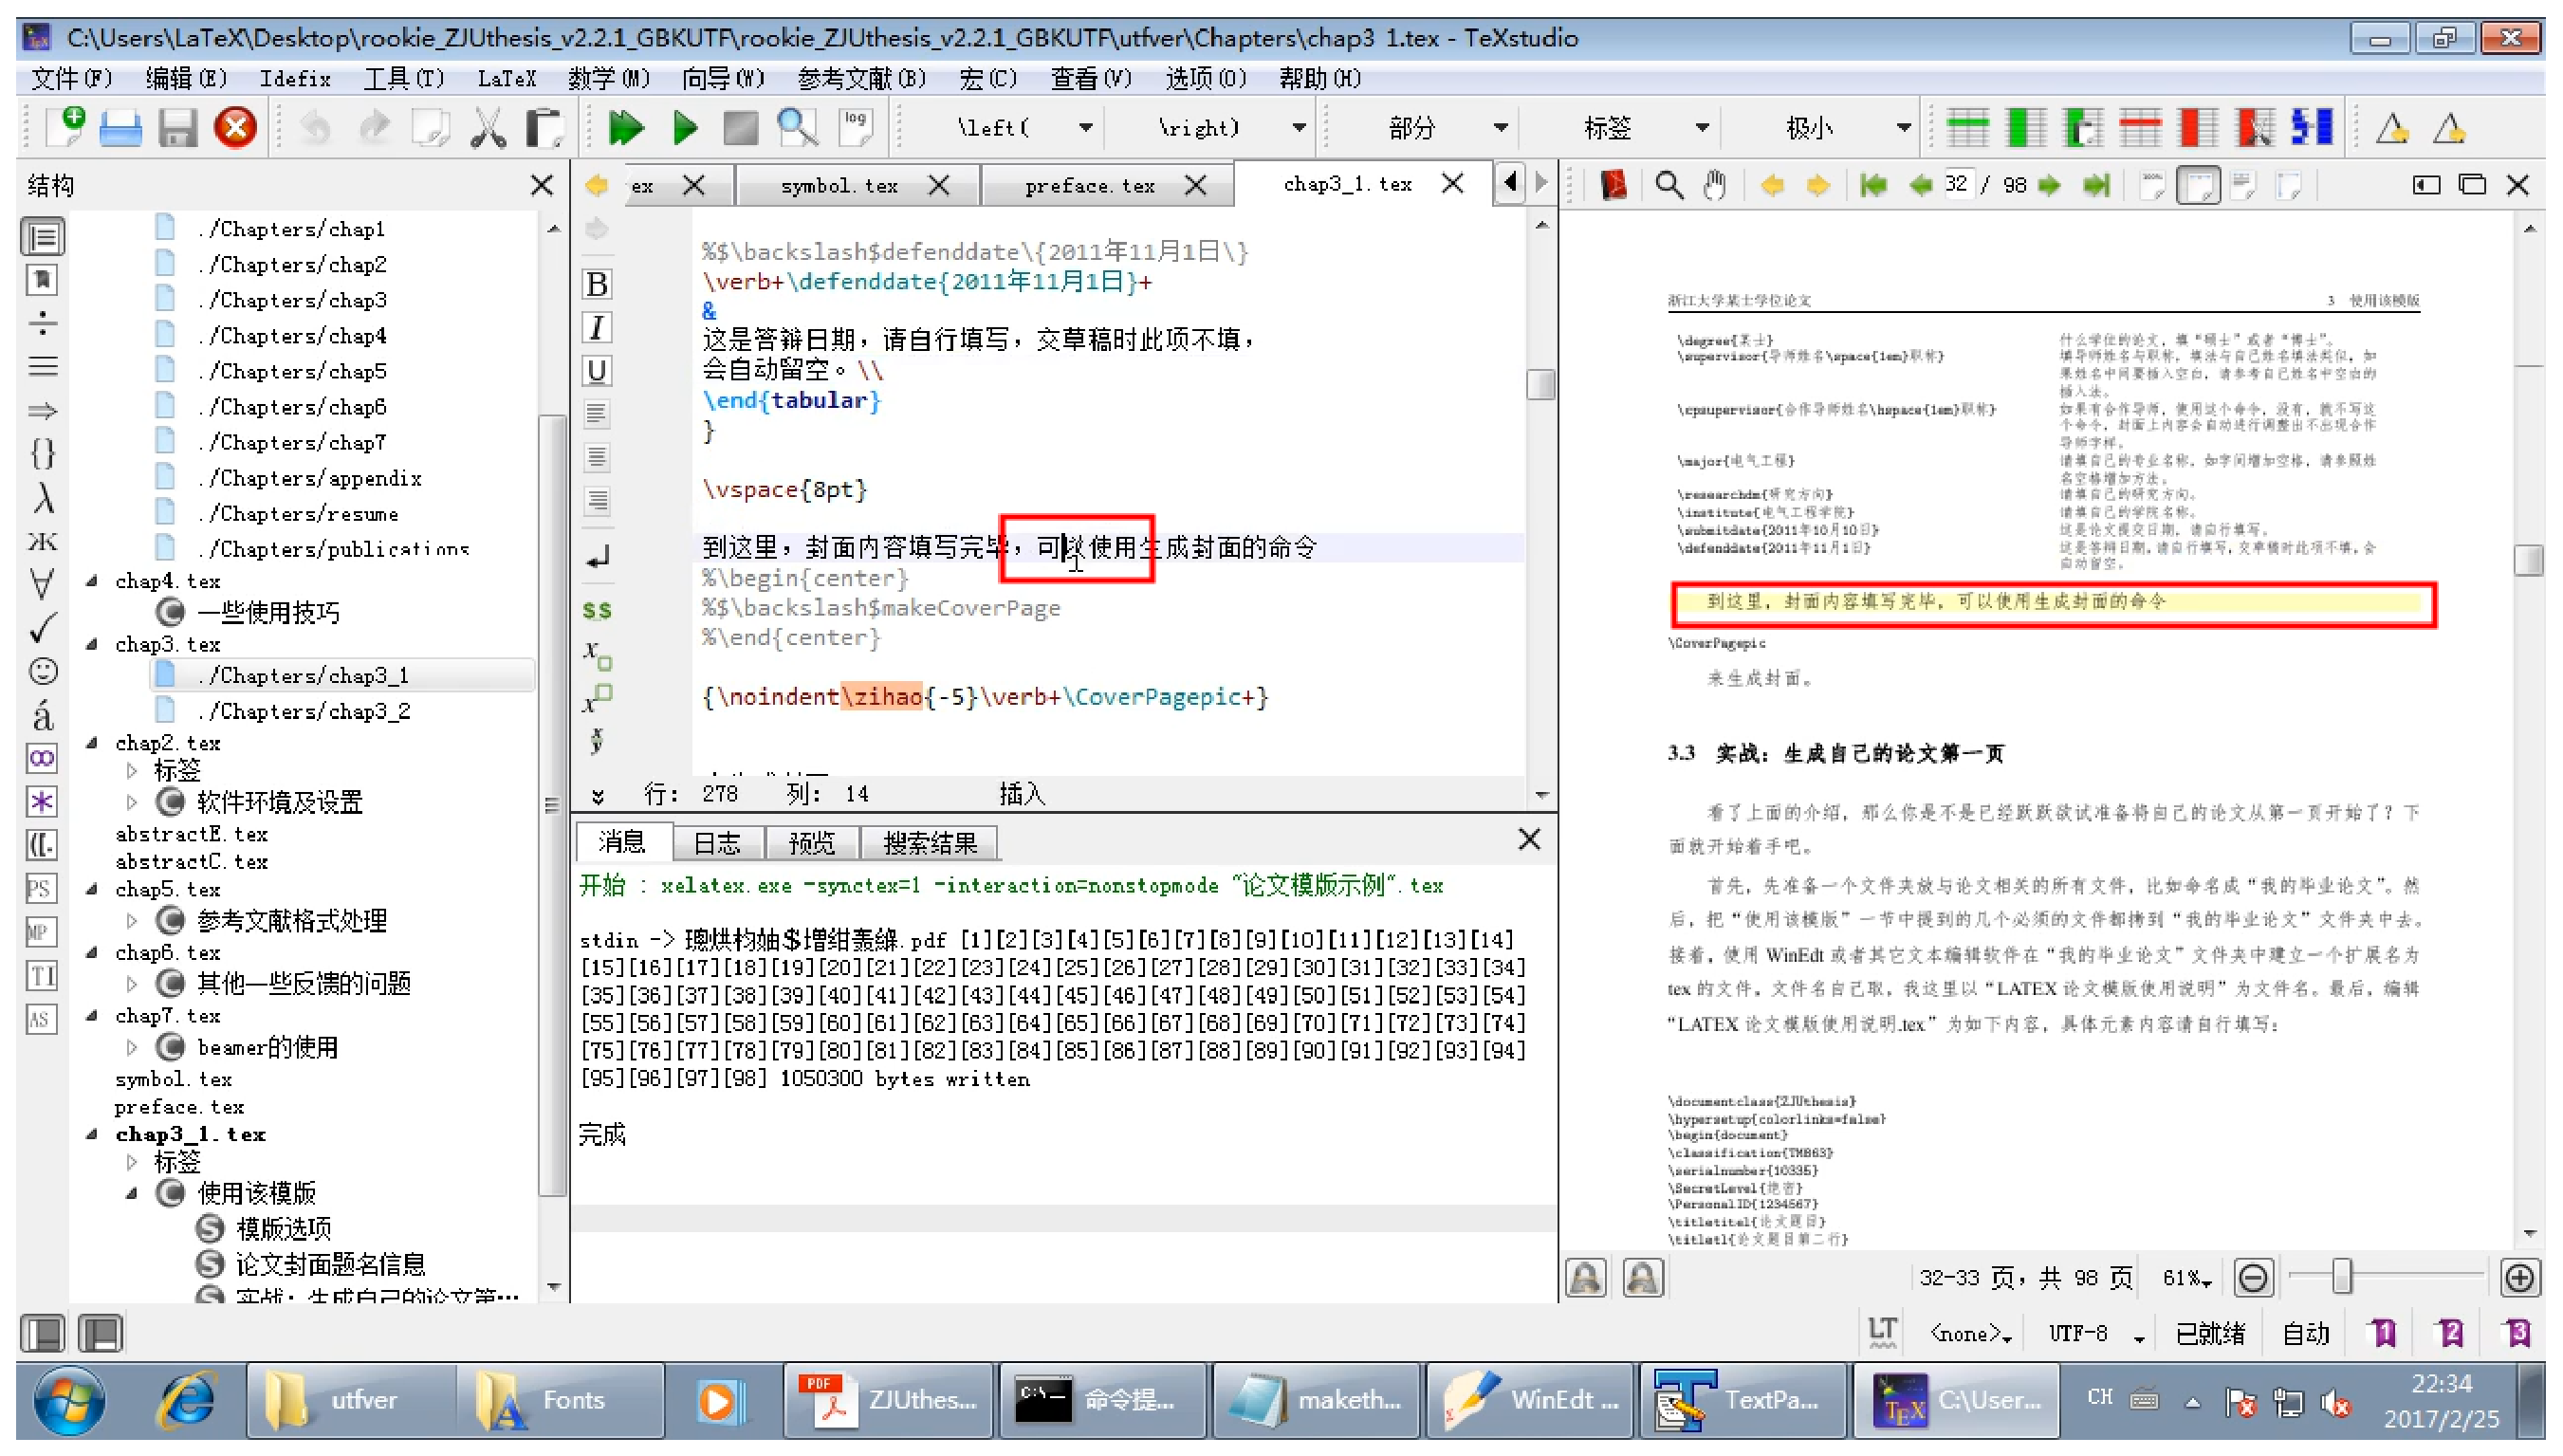
\includegraphics[width=\textwidth]{./Pictures/textopdf.eps}\\
	\caption{TeXstudio中从tex源码跳转到pdf}
	\label{textopdf}
\end{figure}